%% nanicolle-doc-zh.tex
%% Copyright 2016--2020 Yuchang Yang < yang.yc.allium@gmail.com >
%
% This work may be distributed and/or modified under the
% conditions of the LaTeX Project Public License, either version 1.3c
% of this license or (at your option) any later version.
% The latest version of this license is in
%   http://www.latex-project.org/lppl.txt
% and version 1.3c or later is part of all distributions of LaTeX
% version 2005/12/01 or later.
%
% This work has the LPPL maintenance status `maintained'.
% 
% The Current Maintainer of this work is Yuchang Yang.
%
% This work consists of:
%   - the class file: [nanicolle.cls];
%   - the illustration files: [point.pdf, ChinaMainland.pdf, Dongguan.pdf];
%   - the manual files: [nanicolle-doc-zh.tex, nanicolle-doc-zh.pdf, 
%                        nanicolle-doc-en.tex, nanicolle-doc-en.pdf, README.md];
%   - the example files: [nanicolle-ex-zh.tex, nanicolle-ex-zh.pdf,
%                         nanicolle-ex-en.tex, nanicolle-ex-en.pdf].
%%

% arara: xelatex
% arara: xelatex

\documentclass[a4paper]{ctexart}
	\CTEXsetup[format={\Large\bfseries}]{section}

\usepackage[top=32mm,bottom=32mm,textwidth=39em]{geometry}
\usepackage{marvosym}
\usepackage{metalogo}
\usepackage{rulerbox}
\usepackage{tikz}
\usepackage{color}
	\definecolor{mikudark}{RGB}{19, 149, 139}
\usepackage{array}
	\newcolumntype{+}{>{\global\let\currentrowstyle\relax}}
	\newcolumntype{^}{>{\currentrowstyle}}
	\newcommand{\rowstyle}[1]{\gdef\currentrowstyle{#1}#1\ignorespaces}
\usepackage{enumitem}
	\setlist[description]{font=\color{mikudark}\bfseries,leftmargin=2em}
\usepackage{multicol}
	\setlength\columnsep{3em}
	\setlength\columnseprule{0.4pt}
\usepackage{adjustbox}
\newbox\mynmy
\sbox\mynmy{%
	\smash{\raisebox{-5mm}{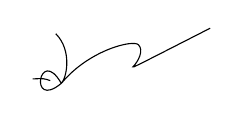
\begin{tikzpicture}[x=7mm,y=7mm]
	\draw (0,1.2)
		.. controls (0.3,0.9) and (0.2,0.4) .. (0.1,0.3)
		.. controls (-0.5,-0.2) and (-0.3,1) .. (0.1,0.3)
		.. controls (0.1005,0.299) .. (0.11,0.31)
		.. controls (0.6,0.9) and (1.4,1.1) .. (1.5,1)
		.. controls (1.6,0.9) and (1.5,0.7) .. (1.4,0.6)
		.. controls (1.39,0.58) .. (2.8,1.3);
	\draw (-0.42,0.38) .. controls (-0.22,0.39) .. (-0.1,0.35);
	\end{tikzpicture}}}}

\makeatletter
\let\url\texttt
\let\emph\textbf
\let\pkgname\textsf
\let\uppercase\relax
\def\@fnsymbol#1{\ifcase#1\or*\or\Letter\fi}
\def\qtimes{\ensuremath{\times}}
\def\tab{\penalty-\@ne\kern1pt\raisebox{.2ex}{\ensuremath{\rightarrow}}\kern1pt\relax}
\def\uspace{\textvisiblespace\allowbreak}
\def\@lan{\raisebox{.2ex}{\ensuremath{\langle}}}
\def\@ran{\raisebox{.2ex}{\ensuremath{\rangle}}}
\def\param#1{\textrm{\@lan\textit{#1}\@ran}}
\def\stopurl{\rlap{\char00}} % WHY URL IS TO GRAB EVERYTHING IT SEES?
\long\def\cmd#1{{\ttfamily\color{mikudark}#1}}
\long\def\pbox#1{\leavevmode\parbox{.86\linewidth}{\cmd{#1}}\kern-.03\linewidth}
\long\edef\[#1\]{$$\noexpand\pbox{\noexpand\raggedright#1\par}$$}
\catcode`\$=\active 
\def\check@nextchar{%
	\if\@nextchar、\unskip\fi
	\if\@nextchar,\unskip\fi
	\if\@nextchar:\unskip\fi
	\if\@nextchar;\unskip\fi
	\if\@nextchar。\unskip\fi}
\def$#1${\CJKecglue\cmd{#1}\CJKecglue
	\futurelet\@nextchar\check@nextchar}
\newcount\itemcnt
	\def\clearcnt{\itemcnt\z@}
	\def\@black#1{{\color{black}\rmfamily#1}}
	\def\@theitem{\advance\itemcnt\@ne\@black{\romannumeral\the\itemcnt.\space}}
	\def\@blackperiod{\@black{。}\@gobble}
	\def\@blackcolon{\@black{;}\penalty-\@ne}
	\def\ritem#1{\@theitem#1\@ifnextchar*\@blackperiod\@blackcolon}
\makeatother

\title{植物标本标签文档类\pkgname{nanicolle}%
	\footnote{本项目的Github仓库地址为\url{https://github.com/Mikumikunisiteageru/nanicolle}\stopurl 。}}
\author{杨宇昌%	
	\footnote{电子邮箱为\url{yang.yc.allium@gmail.com}\stopurl 。}%
	\qquad\box\mynmy\kern-1cm}
\date{2020年8月31日\qquad ver.~2.03y}

%%%%%%%%%%%%%%%%%%%%%%%%%%%%%%%%

\begin{document}

\xeCJKsetup{CJKglue={\hskip0pt}}

\maketitle

\parskip=1ex\relax

植物标本是经处理能够长期保存的植物材料。它们是植物居群的样本,通过标本可以了解植物居群。由于植物材料本身并不能完整地反映居群的所有重要信息,标本采集者需要作出补充并记录成\emph{采集标签},与标本一同保存。植物分类学者可以研究判定标本对应居群所属的物种,其鉴定意见则以\emph{鉴定标签}的形式,附在标本上。

\LaTeX{}文档类\pkgname{nanicolle}可排版植物标本用的中式或西式的采集标签和鉴定标签。中式的两种标签分别由$\string\Collect$命令和$\string\Identify$命令产生。要排版西式的采集标签和鉴定标签,需改用小写的$\string\collect$和$\string\identify$命令,格式和前者大致相同,具体要求和用例见英文文档。本中文文档中所说的标签都默认是中式的。
标签会安排在横向A4尺寸、分为四栏的页面上,可以用A4纸张打印。目前,\pkgname{nanicolle}文档类仅支持\XeLaTeX{}引擎编译。

\pkgname{nanicolle}按 The \LaTeX{} Project Public License (LPPL) 1.3c 许可证\footnote{LPPL 1.3c 许可证的详细内容见\url{http://www.latex-project.org/lppl.txt}\stopurl 。}授权发布。它依赖\pkgname{C\TeX{}}宏集和
	\pkgname{calc}、
	\pkgname{color}、
	\pkgname{geometry}、
	\pkgname{graphicx}、
	\pkgname{listofitems}、
	\pkgname{multicol}\footnote{由于指定 \pkgname{nanicolle} 文档类会间接地构成对 \pkgname{multicol} 宏包的使用,若要将 \pkgname{nanicolle} 用于商业用途,则需要向 \pkgname{multicol} 宏包的作者支付授权费用,详情见该宏包的授权许可证。}、
	\pkgname{xstring}
等宏包。

\parskip=0ex\relax

% \vfill
\tableofcontents\vfill\null

\clearpage

%%%%%%%%%%%%%%%%%%%%%%%%%%%%%%%%

\section{\pkgname{nanicolle}类文档的结构}\label{usage}

一份使用\pkgname{nanicolle}类的文档应是包含以下5部分、文件名以后缀 \texttt{.tex} 结尾的纯文本:
\begin{enumerate}
	\item 载入\pkgname{nanicolle}文档类,即$\string\documentclass[\param{选项}]\{nanicolle\}$。
		其中,$\param{选项}$控制文档的行为,例如$nomap$可禁用采集标签中的地图,$autoduplicate$则能按标本份数重复采集标签;选项超过一个时,其间要用$,$分隔。不需要加载选项时,可写$\string\documentclass\{nanicolle\}$。
	\item 在导言区使用$\string\heading$和$\string\subheading$命令定义定制内容。要在采集标签上方添加统一的标题,可写$\string\heading\{\param{标题}\}$;副标题如需要则可由$\string\subheading\{\param{副标题}\}$命令产生。二者长度均不得超过一行。若跳过此部分,则采集标签上方无标题。
	\item 正文开始,即$\string\begin\{document\}$。
	\item 在正文中使用$\string\Collect$和$\string\Identify$两种命令分别产生采集标签和鉴定标签,每个命令占一行。两种命令的格式分别参见第 \ref{collect} 和第 \ref{identify} 节。
	\item 正文结束,即$\string\end\{document\}$。
\end{enumerate}

%%%%%%%%%%%%%%%%%%%%%%%%%%%%%%%%

\section{用\hbox{}$\textbackslash Collect$命令生成采集标签}\label{collect}

$\string\Collect$命令的格式为
\[%
	\hangindent=2em\relax
	\string\Collect
		\tab\param{记录号}\tab\param{采集人}\tab\param{采集号}%
		\tab\param{采集日期}\tab\param{科名}\tab\param{中文名}%
		\tab\param{学名}\tab\param{照片号}\tab\param{标本份数}%
		\tab\param{产地}\tab\param{经度}\tab\param{纬度}%
		\tab\param{海拔}\tab\param{生境}\tab\param{生活型}%
		\tab\param{体高}\tab\param{胸径}\tab\param{附注}%
\]
当中$\tab$表示水平制表符(U+0009,可按键盘Tab键输入)。每行最多能有一个$\string\Collect$命令;每个$\string\Collect$命令及其所有参数必须出现在同一行中。
某些参数可以为空,但$\tab$都须保留。
以下分别说明诸参数。

\begin{enumerate}
	\item $\param{记录号}$:仅为数据组织方便而设,不在采集标签上出现。
	\item $\param{采集人}$:标本的采集者的姓名。如有多个采集者,应列举姓名,其间可以用顿号分隔;如果要填写采集团队名称,也应注明其成员。此参数不得为空。
	\item $\param{采集号}$:属于$\param{采集人}$中第一个采集者的记录标本采集的序列号码。建议为简单的整数,从1开始递增。
	\item $\param{采集日期}$:采集植物材料的日期,可使用$\param{年}.\param{月}.\param{日}$的阿拉伯数字表示。此参数不得为空。
	\item $\param{科名}$:临时鉴定的科的名称,建议使用中文表示。
	\item $\param{中文名}$:临时鉴定的植物中文名。
	\item $\param{学名}$:临时鉴定的植物学名,建议不带作者引证。当非空时,可用通式$\param{属级部分}\param{种级部分}\param{种下等级部分}$表示。
		其中,$\param{属级部分}$有2类结构:
		\[\clearcnt
			\ritem{\param{属名}}%
			\ritem{\qtimes\param{属名}}*\]
		$\param{种级部分}$有9类结构:
		\[\clearcnt
			\ritem{\uspace sp.}%
			\ritem{\uspace sp.\uspace nov.}%
			\ritem{\uspace\param{种加词}}%
			\ritem{\uspace\qtimes\param{种加词}}%
			\ritem{\uspace aff.\uspace\param{种加词}}%
			\ritem{\uspace aff.\uspace\qtimes\param{种加词}}%
			\ritem{\uspace cf.\uspace\param{种加词}}%
			\ritem{\uspace cf.\uspace\qtimes\param{种加词}}%
			\ritem{\uspace '\param{栽培种名}'}*\]
		当中的$\uspace$表示一个空格(U+0020)。$\param{种下等级部分}$仅当$\param{种级部分}$为结构iii或结构iv时可以非空,此时它有4类结构:
		\[\clearcnt
			\ritem{\uspace subsp.\uspace\param{亚种加词}}%
			\ritem{\uspace var.\uspace\param{变种加词}}%
			\ritem{\uspace f.\uspace\param{变型加词}}%
			\ritem{\uspace '\param{栽培品种名}'}*\]
    此参数中不能用$\string\textit$之类的控制序列手动控制字体样式。
	\item $\param{照片号}$:仅为数据组织方便而设,不在采集标签上出现。
	\item $\param{标本份数}$:标本的同号复份数目,用阿拉伯数字表示。不在采集标签上出现。当文档类的$\param{选项}$包含$autoduplicate$时,每个$\string\Collect$命令将输出$\param{标本份数}$张重复的采集标签。
	\item $\param{产地}$:植物材料的采集地的自然语言表述,要包含完整的省级、县级、乡级行政单元序列和小地点,小地点可参照地标表示,以便考证与回访。此参数不得为空。
	\item $\param{经度}$:植物材料采集地的经度坐标,用十进制的浮点数表示,以角度为单位,不带单位符号,正数为东经,负数为西经。不接受度分秒表示。
	\item $\param{纬度}$:植物材料采集地的纬度坐标,用十进制的浮点数表示,以角度为单位,不带单位符号,正数为北纬,负数为南纬。不接受度分秒表示。
	\item $\param{海拔}$:植物材料采集地的海拔高度,用阿拉伯数字表示,以米为单位,不带单位符号,可以为负数。
	\item $\param{生境}$:植物居群的野外生活环境,如$山地$、$林缘$、$溪边$等,但对于栽培的植物,应填写$栽培$而非具体的生活环境。
	\item $\param{生活型}$:植物居群的生活型,如$乔木$、$灌木$、$藤本$等。
	\item $\param{体高}$:植物居群中个体的典型高度,用阿拉伯数字表示,以米为单位,不带单位符号。
	\item $\param{胸径}$:植物居群中个体的典型胸径,用阿拉伯数字表示,以厘米为单位,不带单位符号。
	\item $\param{附注}$:包含其他在植物标本上无法观察的有价值的信息,如各部的颜色、气味,树皮的纹理,传粉者,植物在当地的俗名、用途、常见程度等。和以上各参数不同,$\param{附注}$是完整的句子,末尾要有标点。
\end{enumerate}

\pkgname{nanicolle}文档类默认在经纬度均非空且经度在东经73--136度间、纬度在北纬17--54度间时在采集标签下方输出地图,以标明该坐标的位置。要禁用这个功能,可以在载入文档类时使用$nomap$选项,见第 \ref{usage} 节。

%%%%%%%%%%%%%%%%%%%%%%%%%%%%%%%%

\section{用\hbox{}$\textbackslash Identify$命令生成鉴定标签}\label{identify}

$\string\Identify$命令的格式为
\[%
	\hangindent=2em\relax
	\string\Identify
		\tab\param{记录号}\tab\param{学名}\tab\param{中文名}%
		\tab\param{鉴定人}\tab\param{鉴定人标准形式}%
		\tab\param{鉴定日期}\tab\param{批注}%
\]
和$\string\Collect$一样,每个$\string\Identify$命令及其所有参数需独占一行。以下就诸参数分别说明。

\begin{enumerate}
	\item $\param{记录号}$:仅为数据组织方便而设,不在采集标签上出现。
	\item $\param{学名}$:正式鉴定的植物学名,须带有作者引证,可用通式$\param{属级部分}\param{种级部分}\param{种下等级部分}\param{作者引证}$表示。此参数不得为空。
	\item $\param{中文名}$:与$\param{学名}$相关联的中文种名。
	\item $\param{鉴定人}$:标本鉴定者的姓名。
	\item $\param{鉴定人标准形式}$:标本鉴定者的姓名在分类学上约定的标准形式。此参数与$\param{鉴定人}$不得同时为空。
	\item $\param{鉴定日期}$:鉴定标本的日期,格式同$\param{采集日期}$。此参数不得为空。
	\item $\param{批注}$:需另外表明的分类学意见。和以上各参数不同,$\param{批注}$是完整的句子,末尾要有标点。
\end{enumerate}

不同于$\string\Collect$命令,$\string\Identify$命令不带$\param{标本份数}$参数,故每个$\string\Identify$命令固定地输出一张鉴定标签。要输出重复的鉴定标签,只能手动复制命令所在的行。

%%%%%%%%%%%%%%%%%%%%%%%%%%%%%%%%

\section{其他问题}

\subsection{用电子表格软件储存原始数据}

$\string\Collect$与$\string\Identify$之所以不遵照\LaTeX{}惯例而用制表符$\tab$作为参数的定界符,其用意是使得原始数据可以储存电子表格(Spreadsheet)软件\footnote{Microsoft Office Excel 便是一种电子表格软件。}中。当纯文本粘贴到电子表格中时,换行符分隔各行,制表符分隔行内各列。当电子表格的内容粘贴为纯文本时,各行由换行符分隔,行内各列由制表符分隔(形成TSV格式)。事实上,这种规定允许储存于电子表格中的原始数据可以直接为\XeLaTeX{}引擎所读取。具体来说,可以建立一个形如表 \ref{table} 的电子表格来储存原始数据。
\begin{table}[htbp]
	\centering
	\begin{tabular}{|+c|*{8}{^c|}}
		\hline
		\rowstyle{\bfseries} 命令 & 记录号 & 采集人 & 采集号 & 采集日期 & 科名 & 中文名 & 学名 & \ensuremath{\cdots} \\\hline
		\string\Collect & 1 & \ensuremath{\cdots} & \ensuremath{\cdots} & \ensuremath{\cdots} & \ensuremath{\cdots} & \ensuremath{\cdots} & \ensuremath{\cdots} & \ensuremath{\cdots} \\\hline
		\string\Collect & 2 & \ensuremath{\cdots} & \ensuremath{\cdots} & \ensuremath{\cdots} & \ensuremath{\cdots} & \ensuremath{\cdots} & \ensuremath{\cdots} & \ensuremath{\cdots} \\\hline
		\string\Collect & 3 & \ensuremath{\cdots} & \ensuremath{\cdots} & \ensuremath{\cdots} & \ensuremath{\cdots} & \ensuremath{\cdots} & \ensuremath{\cdots} & \ensuremath{\cdots} \\\hline
	\end{tabular}
	\caption{储存采集标签原始数据的电子表格示例}\label{table}
\end{table}
这样,电子表格中的若干行被选中并复制到纯文本环境下后便自动转换成了$\string\Collect$或$\string\Identify$命令要求的格式。而电子表格中的原始数据库在这些命令所要求的参数外还能储存更丰富的信息,这些额外信息会被$\string\Collect$或$\string\Identify$命令忽略,不影响标签的内容。

\subsection{PDF文件的打印设置}

编译得到的PDF文件最终要用打印机打印并裁剪,成为可实际使用的标签。打印机的可打印范围一般比纸面小,故打印机通常默认将文件略为缩小。而\pkgname{nanicolle}采用A4纸横向四列布局,按这样印出来的线条裁切,便会出现两侧的标签宽、中间的标签窄的情形。为避免这种问题,打印PDF文件时应选中“使用原始页面大小”选项。

%%%%%%%%%%%%%%%%%%%%%%%%%%%%%%%%

\section{完整实例}

以下是\pkgname{nanicolle}类的一份文档实例,即包中的 \texttt{nanicolle-ex-zh.tex} 文件。实际的行和左侧的行号是对应的,每个$\string\Collect$或$\string\Identify$命令和其所有参数均在同一行中,折行只是便于展示。定位至文件所在目录并运行 \texttt{xelatex nanicolle-ex-zh},编译完后即可得到 \texttt{nanicolle-ex-zh.pdf}(图 \ref{example})。
\begingroup
\catcode`\^^I\active\let^^I\tab
\catcode`\ \active\let \uspace
\[%
\clearcnt
\everypar={\hangindent=2em\relax\advance\itemcnt1\relax%
\leavevmode\llap{\number\itemcnt\quad}}
\xeCJKsetup{CJKecglue={}}
\linespread{1.23}\selectfont
\string\documentclass[autoduplicate]\string{nanicolle\string}\par
\string\begin\string{document\string}\par
\string\Collect	724	杨宇昌	5358	2017.5.29	报春花科	粉报春	Primula farinosa	5992	1	内蒙古自治区赤峰市阿鲁科尔沁旗新民乡西拉沐伦大峡谷园区	117.574461	43.136042	918.6	沼泽化草甸	直立草本	0.2		花粉红色,花梗与花萼常被白粉;与天山报春 \string\textit\string{Primula nutans\string} 混生。\par
\string\Identify	78	Allium chrysanthum Regel	野葱	杨宇昌		2017.12.7	\par
\string\Collect	1997	杨宇昌	5731	2018.5.8	忍冬科	苦糖果	Lonicera fragrantissima subsp. standishii	7609	2	河北省邯郸市武安市管陶乡董家门村西至洞垴途中			1356.0	山坡灌草丛	灌木	3		果实橙红色,味甜微苦。\par
\string\Identify	439	Maianthemum bifolium (L.) F. W. Schmidt	舞鹤草	杨宇昌		2018.12.9	\par
\string\Identify		Idesia polycarpa var. vestita Diels	毛叶山桐子	杨宇昌		2016.5.20	\par
\string\Identify	128	Kandelia obovata Sheue, H. Y. Liu \string& J. W. H. Yong	秋茄树	杨宇昌		2018.3.5	\par
\string\Identify	585	Ulmus lamellosa C. Wang \string& S. L. Chang	脱皮榆	杨宇昌		2019.4.11	\par
\string\end\string{document\string}\par
\]
\endgroup\par

\begin{figure}[htbp]
	\centering
	\fboxsep=-.2pt\relax
	\hbox{}\hidewidth\rulerbox{\vbox{\kern-.2pt\hbox{\kern-.2pt\fbox{\includegraphics*[bb=0cm 0cm 14.85cm 21cm]{nanicolle-ex-zh.pdf}}\kern-.2pt}\kern-.2pt}}\hidewidth\hbox{}\par
	\caption{样例PDF文件 \texttt{nanicolle-ex-zh.pdf} 的前2栏(左半页)}\label{example}
\end{figure}

%%%%%%%%%%%%%%%%%%%%%%%%%%%%%%%%

\section{更新日志}
\begin{multicols}{2}
\begin{description}[style=nextline]
	\parskip=0pt
	\obeylines
	\item[ver. 2.03y (2020.8.31)]
		更精细地控制分类码,参数中允许不加转义地使用$\%$、$\$$、$\#$、$\string~$等字符,参数外允许$\tab$在行首缩进代码。
		修正中式采集标签中$\param{学名}$栏泄漏段落形状的漏洞。
		修正作者引证中$ex$排成$et$的错误。
	\item[ver. 2.02 (2020.7.8)]
		修正负经纬度值不能解析的错误。
		中式采集标签的参数取消长度限制。
		恢复西式采集标签排版功能。
		新增西式标签样例和英文文档。
	\item[ver. 2.01 (2019.9.27)] 
		再改进采集标签中下划线表的实现。
		支持在附注等参数中直接用\LaTeX{}命令如 $\string\textit$ 等控制字体样式。
		合并解析拉丁学名的两处代码,允许在采集标签的学名后引证作者。
	\item[ver. 2.00 (2019.4.28)] 
		全部代码重构,打包为文档类,重新命名为\pkgname{nanicolle}。
		新增地图自定义与自动选择功能。
		暂时删去西式采集标签排版功能。
		删去标本条码标签排版功能。
		删去某植物园的建筑地图。
		正式发布于CTAN和Github上。
	\item[ver. 1.14 (2018.12.2)]
		新增 $\textbackslash ifinternal$ 开关,以快速控制条码、照片号、标题等。
	\item[ver. 1.13 (2018.9.15)]
		改进采集标签中下划线表的实现。
		修正地图中的国界错误。
		\sout{采集标签中增加某植物园建筑地图。}
		缩减采集标签中的悬挂缩进量。
		代码模块化。
	\item[ver. 1.12 (2018.5.15)]
		优化拉丁学名断行位置。
		调整标本条码标签的段落样式。
	\item[ver. 1.11 (2018.3.28)]
		调整原始数据结构。
		鉴定标签中增加命名人标准缩写。
	\item[ver. 1.10 (2018.2.9)]
		采集标签中增加东莞市镇街地图。
	\item[ver. 1.09 (2018.1.28)]
		\sout{实现标本条码标签排版。}
	\item[ver. 1.08 (2017.10.31)]
		采集标签中增加经度 \ensuremath{73\mbox{--}136\,^\circ\mathrm E}、纬度 \ensuremath{17\mbox{--}54\,^\circ\mathrm N}范围的地图。
	\item[ver. 1.07 (2017.10.22)]
		采集标签与鉴定标签中增加条码。
		实现带有尼泊尔分区地图的西式采集标签排版,用于2017年中国—尼泊尔联合植物考察。
	\item[ver. 1.06 (2017.10.21)]
		采集标签中增加标题。
	\item[ver. 1.05 (2017.7.4)]
		页面布局由A4纸纵向双栏改为横向四栏,字号相应缩小,用途更广。
		改进水平切割线的样式。
	\item[ver. 1.03 (2017.7.2)]
		参数改用制表符分隔,方便操作。
		% 此版本曾发布于Github上。
	\item[ver. 1.02 (2016.8.6)]
		\sout{新造某生僻字。}
	\item[ver. 1.01 (2016.8.3)]
		实现采集标签与鉴定标签排版功能。
\end{description}
\end{multicols}

\end{document}
